\documentclass[a4paper,12pt,leqno,titlepage]{article}
\usepackage{hyperref} %linkitys
\usepackage{graphicx}
\usepackage{listings}
\usepackage{moreverb}
\usepackage{amsmath}
\usepackage{amsthm}
\usepackage[finnish]{babel}
\usepackage{ucs}
\usepackage[utf8x]{inputenc}
\usepackage{amssymb}
%\usepackage{harvard}
%\usepackage{authordate1-4}
\usepackage[sorting=none]{biblatex}

\usepackage{pgfplots}
%\pgfplotsset{width=7cm}%,compact=1.10}

\widowpenalty=1000
\clubpenalty=1000

\setlength{\parskip}{2ex plus 2ex minus 1ex}

%\usepackage[comma,authoryear,numbers]{natbib}
\newcommand{\R}{\mathbb{R}} %lukujoukkosymbolit
\newcommand{\C}{\mathbb{C}}
\newcommand{\Q}{\mathbb{Q}}
\newcommand{\N}{\mathbb{N}}
\newcommand{\Z}{\mathbb{Z}}
\newcommand{\logM}{\mathcal{M}}
\setlength{\parindent}{0pt} %kappalejakoa
%\setlength{\parskip}{2ex}
\newcommand{\compcent}[1]{\vcenter{\hbox{$#1\circ$}}}
\newcommand{\comp}{\mathbin{\mathchoice
{\compcent\scriptstyle}{\compcent\scriptstyle}
{\compcent\scriptscriptstyle}{\compcent\scriptscriptstyle}}}

%\hyphenpenalty=750
%\setlength{\emergencystretch}{1.5 em} % Tavutusasetukset suomen kielelle

\hypersetup{
pdfborder = {0 0 0 0}, %linkkien värejä etc kikkailua
colorlinks = true,
linkcolor = black,
urlcolor = blue,
citecolor = red,
}


\usepackage{lastpage} %sivumäärä alaviitteeseen
\usepackage{fancyhdr}

\pagestyle{fancy}
\cfoot{Sivu \thepage/\pageref{LastPage}}

\bibliography{tutkimussuunnitelma}{}

\begin{document}
\begin{titlepage}
\title{Miten oppilaat kokevat laskupajamuotoisen työskentelyn?} %Laskupajamuotoinen opetus lukiotasolla}
\author{Sandra Luhtaniemi ja Aleksi Markkanen\\
Opiskelijanumerot 013734363 ja 013126382\\
\pageref{LastPage} sivua}
\date{\today}
\end{titlepage}
\maketitle
\pagebreak
\tableofcontents
\pagebreak

\section{Johdanto} %aleksi
Kisälliopetus on uusi ja innovatiivinen tapa opettaa matematiikkaa.
Se eroaa merkittävästi perinteisestä matematiikan opetuksesta, jossa uusi asia luennoidaan ja kotiläksyksi annetaan tehtäviä, jotka liittyvät tunnilla käytyihin asioihin.
Kisälliopetuksessa korostetaan laskemisen merkitystä.
Tehtäviä on tyypillisesti enemmän, ja opettaja kiertelee ja auttaa oppilaita tekemään laskuja.
Neuvonnalla pyritään siihen, että oppilas ymmärtää ongelman ja mahdolliset ratkaisumenetelmät -- ei siis niin, että menetelmät tai ratkaisut vain kerrottaisiin opiskelijalle.
Näin opiskelija itse päätyy ratkaisuun, ja samalla oppii "oikeasti" ymmärtämään käytetyn menetelmän.
Kisälli\-opetuksessa opiskelija pääsee osaksi asiantuntijakulttuurin tapaa toimia.\cite{hautala2012extreme,vihavainen2011extreme}

Helsingin Normaalilyseossa on yksi matematiikan kurssi, joka täyttää kisälliopetuksen piirteet.
Kurssi MAA15S, harjoituskurssi, on suunniteltu käytäväksi samanaikaisesti muiden pitkän matematiikan kurssien kanssa.
Niinpä harjoituskurssilla käsitellään jo opittuja asioita syventävästi.
Kurssin järjestämistapa tarjoaa myös hyvät mahdollisuudet eriyttämiseen.

Harjoituskurssi tapaa kerran viikossa puolen vuoden ajan, ja opiskelija saa siitä yhden kurssisuorituksen.
Kurssilla ei tästä syystä voida tehdä varsinaisen matematiikan kurssin laskuharjoitustehtäviä, vaan kurssin järjestävä opettaja valmistelee laskettavaksi tehtävämonisteen.
Ryhmätyö on sallittua, eikä kurssilla ole tehtäväkiintiötä.
Niinpä kurssin ilmapiiri on hyvä ja rento.
Toisaalta oppilailla saattaa esiintyä motivaatio-ongelmia.
Tutkimuksen tekemisen aikana emme huomanneet tämän muodostuvan suureksi ongelmaksi.

\pagebreak
\section{Teoreettinen viitekehys}
\subsection{Lähikehityksen vyöhyke}
Psykologi Les Vygotskin teoria lähikehityksen vyöhykkeestä esittää, että henkilön toimiessa häntä itseä kokeneemman ohjaajan vaikutuspiirissä, hän kykenee suorituksiin, jotka ylittävät hänen nykyisen eli aktuaalisen tieto- ja taitotasonsa. Vygotskin näkemyksen mukaan henkilön aktuaalisen taitotason ja potentiaalisen taitotason väliin sijoittuu lähikehityksen vyöhykkeeksi nimitetty tila, missä henkilö kykenee ympäristön vaikutuksen ansiosta hänen potentiaalisen taitotasonsa mukaisiin saavutuksiin.\cite{vygotsky1978mind}
\subsection{Scaffolding}
Scaffolding on syväoppimiseen tähtäävä lähikehityksen vyöhykkeen pedagoginen sovellus. Siinä opettaja haastaa opiskelijan tekemään hieman hänen aktuaalista taitotasoaan vaativampia tehtäviä, jotka opiskelija tekee opettajan ohjauksessa. Oppiminen on tehokkaampaa ja syvempää, kuin jos tehtävä olisi liian haasteellinen tai selvästi hänen taitotasoaan alempana. Ideana on, että ohjaaja johdattelee opiskelijan ratkaisemaan tehtävän itse, ja välttää kaikin tavoin ratkaisemasta sitä hänen puolestaan. Yksi scaffoldingin tavoitteita on, että opiskelija vähitellen kehittäisi itselleen opiskelu- ja ongelmanratkaisustrategioita. Keskeistä on myös, että opiskelija oppii paitsi vastaamaan, myös esittämään kysymyksiä.\cite{kirschnerswellerclark}
\subsection{Ongelmaperustainen oppiminen}
Näistä löytyy selvä kytkös ongelmaperustaiseen oppimiseen. Ongelmaperustainen oppiminen on pedagoginen suuntaus, joka tarjoaa kiinnostavan lähesty\-mistavan myös matematiikan opetukseen. Ongelmaperustaisessa oppimisessa opiskelija ratkoo ongelmia, missä hänen on sovellettava laajasti aikaisemmin hankittua teoriapohjaa. Hänelle ei välttämättä ole täysin selvää, mitä eri tekniikoita ratkaisemisessa on sovellettava. Toinen ongelmaperustaisen oppimisen lähestymistapa on tarjoilla teoria ongelman muodossa: opis\-kelija saa eteensä ongelman, ja hänen on löydettävä sen ratkaisemiseen vaadittava teoria ja heuristiikat.\cite{schoenfeld}
\subsection{Kisälliopetus}
Laskupajaopetus voidaa nähdä sovelluksena niin sanotusta kisälliopetuk\-sesta. Kisälliopetus on ajankohtainen tutkimusaihe, jota on tutkittu muun muassa Helsingin yliopistossa yliopistotason kursseilla. Matematiikan opiske\-lussa tehtävien tekeminen on ratkaisevassa asemassa ja sitä ei voi oppia pelkästään lukemalla tai kuuntelemalla. Lukio-opetuksessakin painotus on vahvasti tehtävien tekemisessä. Pyritään siihen, että opiskelijat ratkoisivat mahdollisimman paljon tehtäviä. Tehtävien pedagoginen hyöty ja potentiaali jää kuitenkin käyttämättä, mikäli ne ovat niin haasteellisia opiskelijan taitoihin nähden, että niiden tekeminen ei yksinkertaisesti onnistu. Mate\-ma\-tiikka on kuin lohikäärme, jonka kanssa tulee taistella, mutta taitavinkin soturi on joskus tarvinnut mestarin.
\subsection{Matematiikkapelko}
\textbf{...tähän}

\pagebreak
\section{Tutkimustehtävä ja tutkimuskysymykset}
Tutkimuksemme tutkimustehtävän oli selvitää, kuinka pajatyöskentely sopii lukio-opintojen yhteyteen.
Halusimme saada oppilaiden näkemykset esiin.
Niinpä emme halunneet tutkia harjoituskurssin vaikutusta muiden kurssien arviointiin, vaan kysyimme oppilaiden mielipiteitä harjoituskurssin hyödyllisyydestä.
Tutkimuskysymykseksemme muodostui siis seuraava:
\textbf{Kuinka hyödylliseksi lukion oppilaat kokevat laskupajatyöskentelyn?}

\section{Tutkimuksen toteutus} %aleksi
Päätimme käyttää laadullista tutkimusstrategiaa aineistoa kootessa.

Jaoimme laskupajassa läsnäolleille opiskelijoille ($n=19$) kyselylomakkeet, ja opiskelijat arvioivat seitsemää väitettä sekä Likert-asteikolla että sanallisesti.
Lomakkeessa oli myös viisi avointa kysymystä.

Oppilaat arvioivat seuraavia väittämiä:
\begin{itemize}
\item Harjoituskurssi on parantanut menestystäni muilla matematiikan kursseilla.
\item Tunnen nykyään osaavani ja ymmärtäväni matematiikkaa paremmin.
\item Harjoituskurssi on lisännyt itsevarmuuttani matematiikan osaamisen suhteen.
\item Harjoituskurssista on ollut minulle hyötyä.
\item Saan harjoituskurssilla apua tehtävien ratkaisemiseen.
\item Harjoituskurssilla on mukavaa.
\item Saan harjoituskurssilla tehtyä sellaisiakin tehtäviä, joita en itenäisesti osaisi tehdä.
\end{itemize}
Lomakkeessa oli seuraavat avokysymykset:
\begin{itemize}
\item Saatko sellaista apua, mitä kaipaat? Minkälaista apua kaipaat matematiikassa?
\item Mitkä ovat vahvuutesi matematiikassa? Entä heikkoudet?
\item Kuinka harjoituskurssia voisi parantaa?
\item Miksi päätit osallistua tälle kurssille?
\item Toivoisitko vastaavanlaista kurssia myös myöhempien opintojen aikana?
\end{itemize}
\begin{comment}
Haastattelimme myös harjoituskurssin opettajaa.
\textbf{Tämä pitäisi vielä tehdä..}
\begin{itemize}
\item Miten autat oppilasta löytämään ratkaisun?
\item Millainen on tyypillinen laskupajan asiakas?
\item Onko laskupaja yleensä ollut suosittu?
\item Minkälaisille opiskelijoille laskupaja on suunnattu?
\item Kuinka hyödylliseksi koet laskupajan?
\end{itemize}
\end{comment}
\section{Tutkimustulokset}
Tunnistimme aineistostamme eri oppilastyyppejä.
Kaikki haastatellut oppilaat pitivät harjoituskurssia hyödyllisenä.
Syyt kuitenkin vaihtelivat; suuri osa ($n=9$) piti kurssia hyödyllisenä sen kertaavan luonteen vuoksi.
Neljän opiskelijan mielestä kurssilla on opittu myös uusia asioita, muun muassa laskimen käyttötaitoa.
Kuusi opiskelijaa ei vastannut kysymykseen.
Hyvänä ominaisuutena pidettiin myös sitä, että apua ja neuvontaa on saatavilla.

\begin{figure}[h!]
\centering
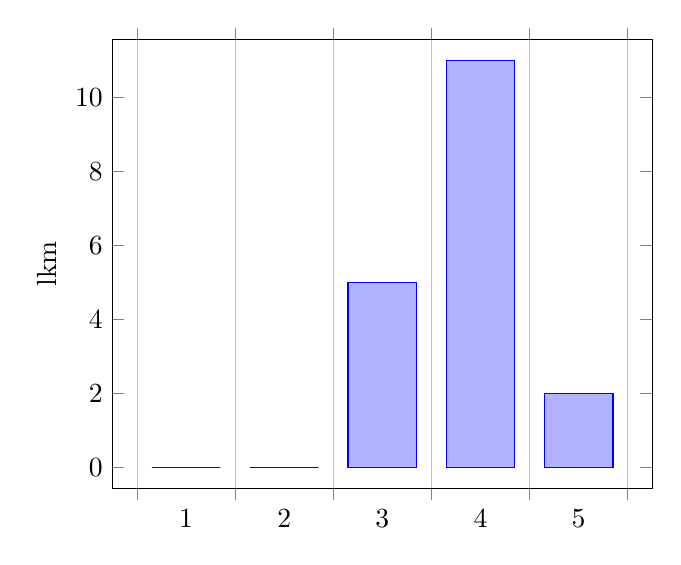
\begin{tikzpicture}
\begin{axis}[x tick label 
style={/pgf/number format/1000 sep=}, ylabel=lkm, enlargelimits=0.05, legend style={at={(0.5,-0.15)}, anchor=north,legend columns=-1},ybar interval=0.7]
\addplot coordinates {(1,0) (2,0) (3,5) (4,11) (5,2) (6,0)}; % miksei piirrä vikaa asiaa? :3
\end{axis}
\end{tikzpicture}
\caption{``Harjoituskurssista on ollut minulle hyötyä.''}
\end{figure}

\subsection{Kisälliopetus}
Kurssi toteuttaa kisälliopetuksen piirteet opiskelijoiden vastauksien mukaan hyvin.
Suurin osa opiskelijoista ($n=12$) kiitteli vastauksissaan sitä, että apua on saatavilla hyvin.
Loput ($n=7$) opiskelijat eivät kommentoineet vastausta, mutta olivat jokseenkin samaa mieltä tai täysin samaa mieltä siitä, että kurssilla saa apua hyvin.

\begin{figure}[h!]
\centering
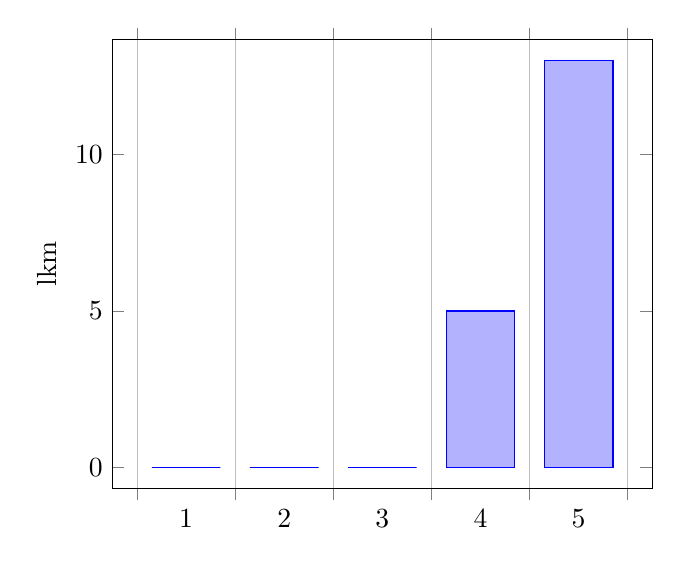
\begin{tikzpicture}
\begin{axis}[x tick label 
style={/pgf/number format/1000 sep=}, ylabel=lkm, enlargelimits=0.05, legend style={at={(0.5,-0.15)}, anchor=north,legend columns=-1},ybar interval=0.7]
\addplot coordinates {(1,0) (2,0) (3,0) (4,5) (5,13) (6,0)}; % miksei piirrä vikaa asiaa? :3
\end{axis}
\end{tikzpicture}
\caption{``Saan harjoituskurssilla apua tehtävien ratkaisemiseen.''}
\end{figure}

Myös \emph{scaffolding}-ilmiö esiintyy vastauksissa.

\begin{figure}[h!]
\centering
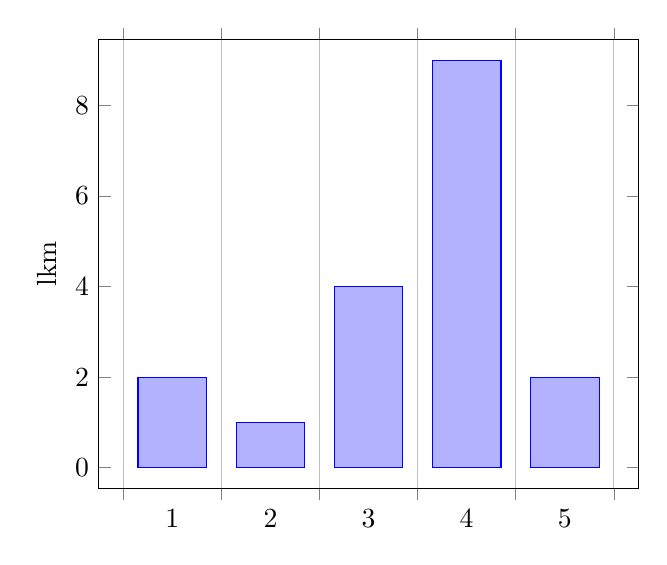
\begin{tikzpicture}
\begin{axis}[x tick label 
style={/pgf/number format/1000 sep=}, ylabel=lkm, enlargelimits=0.05, legend style={at={(0.5,-0.15)}, anchor=north,legend columns=-1},ybar interval=0.7]
\addplot coordinates {(1,2) (2,1) (3,4) (4,9) (5,2) (6,0)}; % miksei piirrä vikaa asiaa? :3
\end{axis}
\end{tikzpicture}
\caption{``Saan harjoituskurssilla tehtyä sellaisiakin tehtäviä, joita en itsenäisesti osaisi tehdä.''}
\end{figure}


\subsection{Opiskelijoiden matematiikkakuva}
Kyselyvastauksista kävi ilmi, että moni opiskelija pitää matematiikkaa enimmäkseen laskemisena.
Lisäksi matemaattisen taidon koetaan kehittyvän harjoittelun avulla.


\subsection{Kurssin vaativuustaso}
Osalle opiskelijoista kurssi oli sopivan vaativa, mutta monet kokivat myös tylsistyvänsä tunnilla.
Tämä tarjoaisi hedelmällisen mahdollisuuden eriyttää opetusta; jos tehtävämonisteita olisi kaksi, kertaava ja syventävä, kurssi palvelisi laajempaa opiskelijajoukkoa.
Koska kurssisuoritukseen riittää vain läsnäolo, valmistaa kurssi myös korkeakoulujen akateemiseen vapauteen; opiskelijalla on vastuu omasta työskentelystään.
Tämä saattaa lisäksi hillitä matematiikkapelkoa, sillä opiskelijalla ei ole paineita suorittaa tiettyä määrää tehtävistä.

\subsection{Miten kurssia voisi kehittää?}


\pagebreak
\section{Pohdintaa}

\subsection{Kehittämisehdotuksia}

\pagebreak

\printbibliography
%\begin{thebibliography}{9}
%\bibitem{xa}
%Hautala, T., Romu, T., Rämö, J., \& Vikberg, T. (2012).
%Extreme apprenticeship method in teaching university-level mathematics. \emph{Proc. of the 12th International Congress on Mathematical Education, International Commission on Mathematical Instruction.}


%\end{thebibliography}


\end{document}
